\section{Mohr-Coulomb-Bruchkriterium}
	\begin{minipage}{\linewidth}
	Verformung = $\Delta$V + $\Delta$Form \\
	$\rightarrow$ bis Bruch linear Elastisch (Hook: $\sigma = \varepsilon \cdot E_{oed}$), danach Mohr-Coulomb \\
	\qquad $\rightarrow$ $E_{oed} = M_E = \frac{4}{3} \cdot G + \kappa$ \\
	\qquad $\rightarrow$ $E_{normal} = \frac{9 \cdot \kappa \cdot G}{3 \cdot \kappa + G}$
	\end{minipage}




\begin{minipage}{0.5\linewidth}
\subsection{Volumetrische ($\Delta$V) Verformung}
	\begin{align*}
		p`				&= \frac{\sigma_1 + \sigma_2 + \sigma_3}{3}	 \\
		\varepsilon_v	&= \frac{\Delta V}{V} = \varepsilon_1 + 2 \cdot \varepsilon_3 \\
		\\
	\end{align*}
\end{minipage}
\begin{minipage}{0.5\linewidth}
\subsection{Deviatorische ($\Delta$ Form aus Schub) Verformung}
	\begin{align*}
		q				&= \sqrt{\frac{(\sigma_1 - \sigma_2)^2 + (\sigma_1 - \sigma_3)^2 + (\sigma_2 - \sigma_3)^2}{2}} \\
		\varepsilon_s	&= \frac{2}{3} \sqrt{\varepsilon_1^2 + \varepsilon_2^2 + \varepsilon_3^2 - (\varepsilon_1 \cdot \varepsilon_2 + \varepsilon_2 \cdot \varepsilon_3 + \varepsilon_1 \cdot \varepsilon_3)} \\
	\end{align*}
	\end{minipage}
	
	
	
	
	\begin{minipage}{0.35\linewidth}
\subsection{Oedometer}
%	\textbf{Visualisierung}
\begin{tabular}{ll}
		$\Delta$Volumen		& $p= \frac{\sigma_1 + 2 \cdot \sigma_3}{3}$ \\
							& $p`= p - u$ \\
							& $\varepsilon_v= \frac{\varepsilon_1}{3}$ \\
		Deviator ($\Delta$Form) &$q`= q = \sigma_1 - \sigma_3$ \\
							& $\varepsilon_s= \frac{2}{3} \cdot \varepsilon_1$ \\
	\end{tabular}
\end{minipage}
\begin{minipage}{0.5\linewidth}
	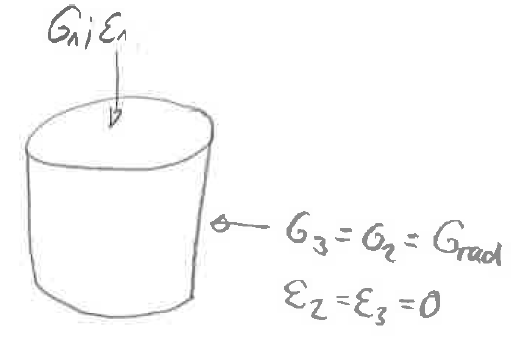
\includegraphics[width=0.5\linewidth]{images/MC1Oed.PNG}
\end{minipage}



\clearpage

\subsection{Ebenerspannungsraum}

\begin{minipage}[t]{0.4\linewidth}
%	\vspace{5cm}
%\textbf{Tau-Sp-Diagramm}
	\begin{align*}
		\tau 		&= c`+ \sigma \cdot tan(\varphi) \\
		\tau		&= b + s`\cdot tan(\beta) \\
		& \rightarrow \varphi = arctan \left(\frac{\Delta \tau}{\Delta \sigma}\right) \\
		& \rightarrow c = \frac{b`}{cos(\varphi)} \\
		& \rightarrow sin(\varphi) = tan(\beta) \\
	\end{align*}
\end{minipage}
\begin{minipage}[t]{0.5\linewidth}
%	\bigskip
	\vspace{\baselineskip}
	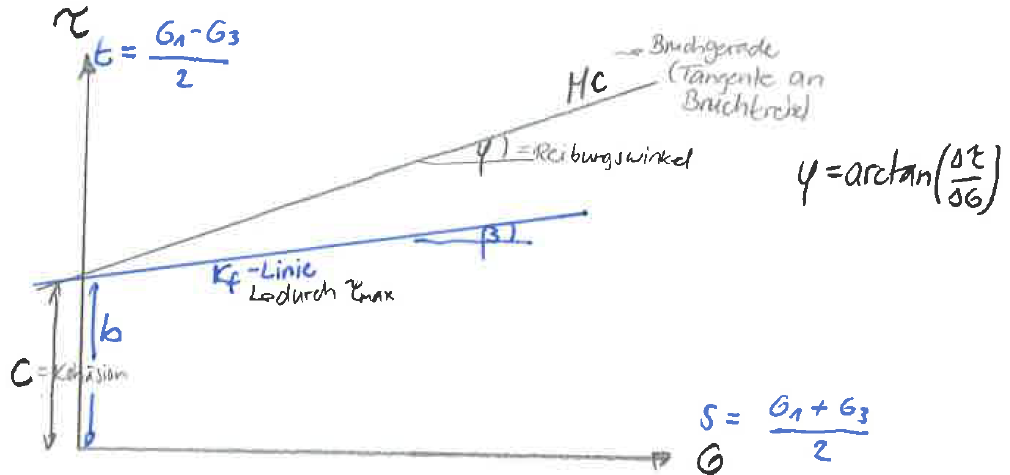
\includegraphics[width=\linewidth]{images/MC2Ebenerspraum.PNG}
\end{minipage}



	

\begin{minipage}{0.6\linewidth}
	\subsection{Dreidimensional}
	\begin{align*}
		q			&= \sigma = M \cdot p + d \\
		M			&= \frac{3 \cdot sin(\varphi)}{\sqrt{3} \cdot cos(\Theta) - sin(\Theta) \cdot sin(\varphi)} \\
					& \rightarrow \Theta = Theta =Winkel der Sp. welche Probe belastet\\
	\end{align*}
\end{minipage}
\begin{minipage}{0.4\linewidth}
	\vspace{\baselineskip}
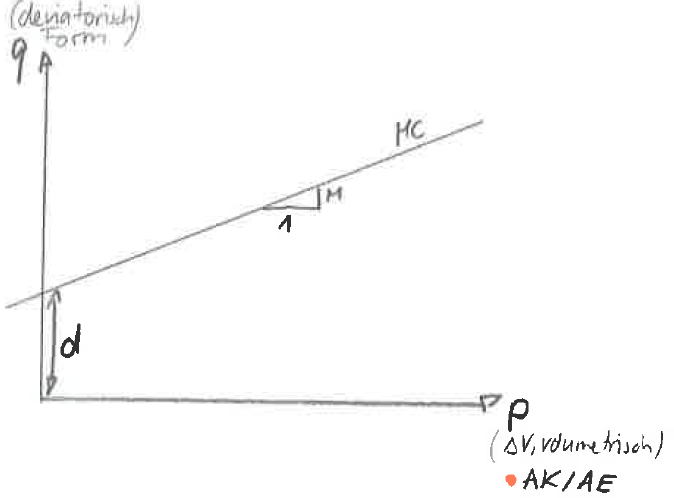
\includegraphics[width=\linewidth]{images/MC33draum.PNG}
\end{minipage}


\begin{minipage}{0.3\linewidth}	
	\subsubsection{Triaxversuch AK}
	\begin{align*}
		M			&= \frac{6 - sin(\varphi)}{3 - sin(\varphi)} \\
		d			&= \frac{6 \cdot c`\cdot cos(\varphi)}{3 - sin(\varphi)} \\
		\Theta		&= 30° = \frac{\pi}{6} \\
	\end{align*}
\end{minipage}
\begin{minipage}{0.5\linewidth}
	\begin{align*}
		\Theta		&= - \frac{\pi}{6}
		\rightarrow \textbf{Kompression}
		&\rightarrow &M_{AK} = \frac{6 \cdot sin(\varphi)}{3 - sin(\varphi)}
		\qquad &d_{AK} = \frac{6 \cdot c`\cdot cos(\varphi)}{3 - sin(\varphi)} \\
		\Theta		&= + \frac{\pi}{6}
		\rightarrow \textbf{Extenssion}
		&\rightarrow &M_{AE} = \frac{- 6 \cdot sin(\varphi)}{3 + sin(\varphi)}
		\qquad &d_{AE} = \frac{- 6 \cdot c`\cdot cos(\varphi)}{3 + sin(\varphi)}
	\end{align*}
\end{minipage}

\begin{minipage}{\linewidth}
	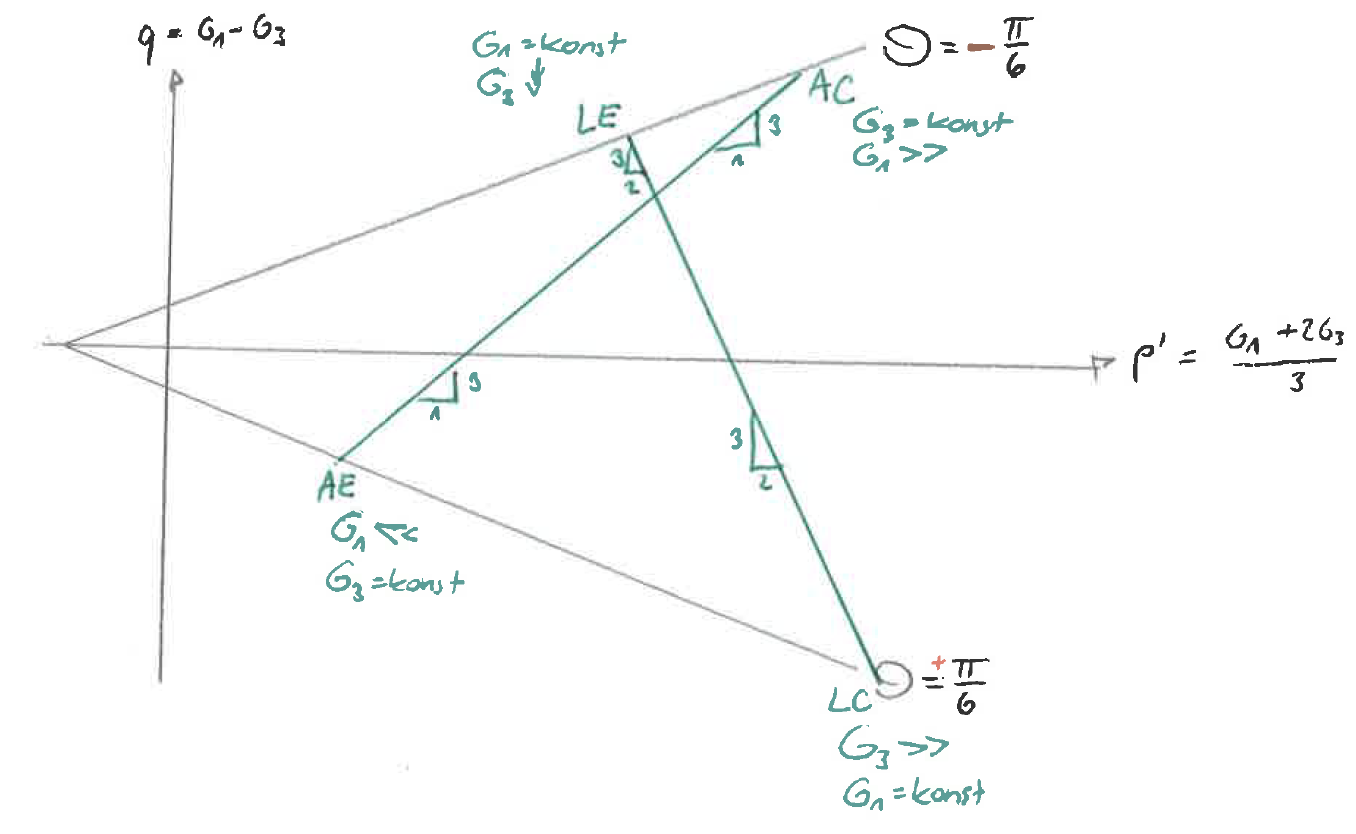
\includegraphics[width=0.8\linewidth]{images/MC4triax.PNG}
\end{minipage}
 \clearpage